\cotefile{156-4}
\scanpage{50}
\mspage{49}

\deleted{\uline{Cont 5} Si $F$ et $G$ sont deux figures disjointes, et \unsure{si} $F'$, \deleted{$G'$\illegible{1} de} subdivision, \inserted{de $F$} alors $F'$ et $G$ sont disjointes.} \margin{\deleted{[\uline{NB} $F'\cap G$ est \unsure{défini|définie} comme, c'est $F'$ et $G$ \uline{\unsure{compatibles|compatible}} qui est notre cas.}}

\deleted{\uline{Cor} Si $F'$ raffine $F$, $G'$ raffine $G$, \deleted{alors} $F$ et $G$ disj. alors $F'$ et $G'$ disjointes.}

\margin{\begin{tikzpicture}[x=.5cm,y=.5cm]\draw(0,0)--(0,1.5);\draw(.13,0)--(.13,1.5);\end{tikzpicture}}\uline{C\deleted{\unsure{ont|ond|ompt|onst}} 5} Soient $F$ une figure, $F'$ une subdivision de $F$. \deleted{\unsure{A}}Alors pour tt figure $G$, $G$ est \unsure{disjoint|disjointe} ; $F$ ssi elle est disjoint\unsure{e} de $F'$

\uline{NB} Il suffit de le poser pour $G$ élémentaire.

Il résulte alors de \deleted{\uline{Cont 4}} C4 que $F'\cup G$ est une subdivision de $F\cup G$.

\uline{Cor} Soient $F$ et $G$ figures disjointes, alors pour $F'\ll F$, $G'\ll F$, $F'$ et $G'$ sont disjointes, et $F'\cup G'\ll F\cup G$. Si $F'$ et $G'$ sont des subd de $F,G$, alors $F'\cup G'$ en est une de $F\cup G$.

\margin{\begin{tikzpicture}[x=.5cm,y=.5cm]\draw(0,0)--(0,1.5);\draw(.13,0)--(.13,1.5);\end{tikzpicture}}\uline{C 6} (Subdivisions induites) Soient $F$ une figure, $F'$ une subdivision de $F$, $G$ une sous-figure de $F$. Alors il existe une unique subdivision $G'$ de $G$, telle que
\[G'\subset F'\]
(subdivision induite) \inserted{et $G'$ est \unsure{formée|formé} des $X\in F'$ telles que $X\ll G$}
\figure{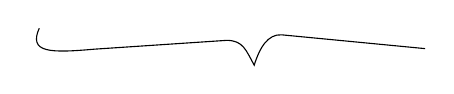
\begin{tikzpicture}[x=1cm,y=1cm,scale=.7]
\draw (0,.25)..controls(-.2,-.2)and(.2,-.2)..(1,-.13)--(3.4,.03)..controls(3.7,.03)and(3.75,-.15)..(3.9,-.42)..controls(4,-.1)and(4.15,.15)..(4.4,.13)--(7,-.12);
\end{tikzpicture}}

\margin{NB \inserted{Double} Transitivité de l'induction. \uline{Notation} $F'|G$}

\margin{\begin{tikzpicture}[x=.5cm,y=.5cm]\draw(0,0)--(0,1.5);\draw(.13,0)--(.13,1.5);\end{tikzpicture}}\uline{C 7} (\deleted{\unsure{D|R}}Recollement \unsure{des|de} subdivisions) Soit $F$ une figure, \deleted{\unsure{chaque|chacune} \illegible{2} \unsure{figure}, \unsure{tt|et}} \inserted{$F_i$ des sous-figures} \deleted{$X\unsure{\in|\subset}$} telles que $F=\bigcup F_i$. Soit, pour tt $i$, $F'_i$ une subdivision de $F_i$, et supposons
